\documentclass[10pt,a4paper,twoside]{article} 
\usepackage[latin1]{inputenc}
\usepackage[english]{babel}
\usepackage{amsmath}
\usepackage{amsfonts}
\usepackage{amssymb}
\usepackage{makeidx}
\usepackage{graphicx}
\usepackage{hyperref}
\usepackage[left=2cm,right=2cm,top=2cm,bottom=2cm]{geometry}
\usepackage{float}
\usepackage{multirow}
\usepackage{verbatim} %for å kommentere ut ting
\usepackage[nottoc,numbib]{tocbibind}
\usepackage[parfill]{parskip} %for avsnitt

\raggedbottom

\usepackage{makeidx}
\makeindex
%symbolliste slutt

\author{Anders Dall'Osso Teigset}
\title{MEDIUM VOLTAGE LOAD BREAK SWITCH WITH AIR AS INTERRUPTING MEDIUM}
\date{December, 2013}


\begin{document}
    \begin{titlepage}
    \begin{center}
    \ \\
    \ \\
    \ \\
    \ \\
    \ \\
    \ \\
    Anders Dall'Osso Teigset \\
    \ \\
    \ \\
    \ \\
    \ \\{\large \bfseries
    MEDIUM VOLTAGE LOAD BREAK SWITCH WITH AIR AS INTERRUPTING MEDIUM\\
    }
    \ \\
    \ \\
    \ \\
    \ \\
    \ \\
    {\large
    Specialisation project\\
    }
    \ \\
    {December, 2013 \\}
    \ \\
    \ \\
    \ \\
    \ \\
    \ \\
    \ \\
    \ \\
    \ \\
    \ \\
    \ \\
    \ \\
    \ \\
    \ \\
    \ \\
    \ \\
    \ \\
    \ \\
    \ \\
    \ \\
    \ \\
    \ \\
    \ \\
    \ \\
    \ \\
    \ \\
    \ \\
    \ \\
    \ \\
    \ \\
   	{\large
   Norwegian University of Science and Technology\\
   Department of Electric Power Engineering\\
    }
   	\ \\
    \ \\
    \ \\
    \ \\
    \end{center}
    \end{titlepage}

%\maketitle
%SummaryNyttige pdf-filer/SF6conduct.pdf
\thispagestyle{empty}
\cleardoublepage
\section*{Acknowledgements}
\setcounter{page}{1}
\pagenumbering{roman}

\cleardoublepage
\section*{Summary}

\cleardoublepage
\setcounter{page}{1}
\pagenumbering{arabic}
\tableofcontents
\cleardoublepage

\section{Introduction}

\cleardoublepage

\section{Theory}
\subsection{Typical switchgear design and interruption sequence}


\subsubsection{Switchgear design and operation} 


\subsubsection{The puffer principle}

   
\subsubsection{Heat transportation in an arc} 


\subsubsection{The difference between air and SF$_6$ as interrupting medium} 



\subsubsection*{Electrical conductivity}


\subsubsection*{Thermal conductivity}


\subsubsection*{Dielectric properties} 


\subsubsection*{Chemical properties}


\subsection{Environmental impacts of SF$_6$ from electrical power industries} 


\cleardoublepage

\section{Method}

\subsection{Test circuit}

Figure \ref{fig:testSwitchRiggEq} illustrates the physical appearance of the test switch. The numbered parts are: 1. Compressed air reservoir (connected to the high voltage supply circuit), 2. Tulip contact, 3. Nozzle, 4. Pin contact, 5. Connection to load circuit, 6. Spring drive mechanism, 7. Electromagnet release mechanism, and 8. Position transducer.

\begin{figure} [H]
\centering
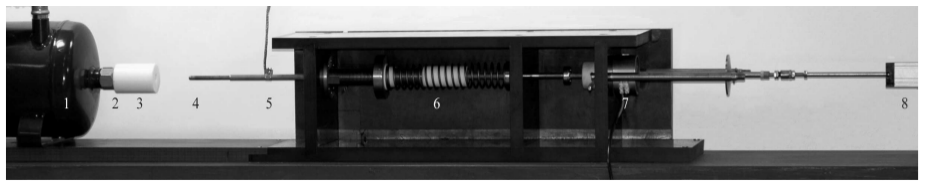
\includegraphics[scale=0.5]{Bilder/Method/switchTest.png}
\caption{The physical appearance of the test switch \cite{bib:AFIMVLBA}.} \label{fig:testSwitchRiggEq}
\end{figure}

Figure \ref{fig:testCurcuit} displays the laboratory test circuit used for the interruption tests. The circuit is designed to supply a 50 Hz / 13.8 kV current. It is possible to shape the TRV by tuning the parameters: L$_1$, L$_s$, R$_1$, R$_d$, and C. The systems' short circuit parameters are R$_{sc}$ and L$_{sc}$. The TRV generated during interruption is set to simulate the standard for a 24 kV / 630 A class from the International Electrotechnical Commission (IEC), which corresponds to:

\begin{itemize}
\item The initial part of the TRV has a rate of rise in recovery voltage (RRRV) of 71 - 73 V / $\mu$s.
	\begin{itemize}
		\item Voltage difference is measured over the first 20 $\mu$s after CZ.
	\end{itemize}
\item The first voltage peak is between 7.0 and 7.4 kV, with a rise time of approximately 96 $\mu$s.
\end{itemize}

\begin{figure} [H]
\centering
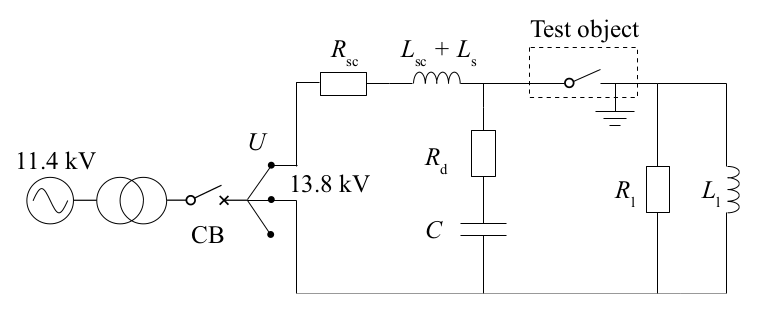
\includegraphics[scale=0.35]{Bilder/Method/circuit.png}
\caption{Circuit used for the interruption test \cite{bib:AFIMVLBA}.} \label{fig:testCurcuit}
\end{figure}

In table \ref{tab:testParameters}, the value of the different test circuit parameters and the corresponding current can be observed. The test is done at currents with an RMS value of 400 A and 630 A. In the entire test the TRV is kept constant up to and including the first voltage peak. In the case of a failed interruption, thermal re-ignition occurs within a few microseconds after CZ.

\begin{table}[H]
\center
\caption{Circuit Parameters and Resulting Current \cite{bib:AFIMVLBA}. }
\begin{tabular}{|c|c|c|c|c|c|}
\hline 
L$_s$ [mH] & L$_1$ [mH] & R$_1$ [$\Omega$] & C [nF] & R$_{d}$ [$\Omega$] & I [A] \\ 
\hline 
14.5 & 138.4 & 35.5 & 74 & 248 & 400 \\ 
\hline 
6.9 & 86.2 & 22.1 & 102 & 198 & 630 \\ 
\hline 
\end{tabular} 
\label{tab:testParameters}
\end{table}

A resistive transducer is measuring the contact position while a Hall Effect current transducer is measuring the current through the test switch. The voltage between the contacts is measured with a parallel resistive / capacitive voltage divider. All measurements are transmitted through optical fibres to a 12 bit resolution transient recorder with a sampling frequency of 2.5 MHz. The pressure in the tank is only measured before each test with an accuracy of 0.01 bar.

\subsection{The switch and contact geometry}



\newpage
\subsection{Procedure}
Interruption tests with CZ occuring both inside and outside the nozzle are carried out. Previous work with a similar setup found that the interruption capability is better outside the nozzle. The first and second CZ is included in this study to provide as much data as possible.

"Inside nozzle" is defined as contact position x = [5?, 25?] mm and "outside nozzle" as x = [35?, 60?] mm at first CZ. Results from zero crossings that occurs in the cylindrical part of the nozzle, between the tulip contact and the start of the funnel-shaped nozzle is discarded. Interruption tests with first CZ either in the start of the funnel-shaped nozzle (x $<$ 5? mm) or in the boundary region between inside and outside the nozzle (x = 25?, 35? mm) are not included in the "interruption success rate graphs", but are presented in tables displaying raw data in appendix \ref{app:rawData}. The first CZ occurred within x $<$ 60 mm and the second CZ occurred for x $>$ 60 mm, as the contact speed during all tests was 5.5 mm/ms $\pm$ 0.5 mm/ms.

When testing the interrupting capabilities, the test procedure for each of the four cases was as follows: 

\begin{itemize}
\item[1.] A pressure level that seems to be in the area of interest is found by performing some initial test interruptions at different pressure levels. This level is kept constant for at least five interruption tests, where the interruptions occurred when the contact pin was outside the nozzle.
\item[2.] If a pressure level results in less than 100\% successful interruptions, at least five new tests with a higher upstream pressure (next level) are conducted. This is repeated until at least one pressure level with five successful interruptions is found.
\item[3.] Then, the pressure is stepped down until 60\% or more of the interruption attempts fail or the lowest possible pressure level is tested.
\end{itemize}

When testing if a connection between the arcing voltage during a successful interruption and an unsuccessful one can be found. A pressure level where the interruption success rate is 50 \% is used. Then five successful interruptions and five unsuccessful interruptions are obtained while the arcing voltage is measured and stored for further use. All the interruptions should occur outside the nozzle. The switching process is filmed by a high speed camera so that the path of the arc can be monitored during the interruption.

The pin is cleaned, polished, and greased between each test to ensure a smooth surface. The contacts and nozzle are replaced regularly to avoid contact wear and nozzle deformation. This is to ensure that the geometry is constant through the whole experiment.
\cleardoublepage

\section{Results}
\subsection{Interruption tests} 


\newpage
\subsection{Arcing voltage}


\newpage
\subsection{Durability of the arcing contacts} \label{sec:durability}



\cleardoublepage

\section{Discussion}
\subsection{The probability of interruption} 


\subsection{Arcing voltage considerations}
 

\subsection{Durability of the arcing contacts} \label{fig:durability}


\newpage
\subsection{Suggestion for further work}
\subsubsection{A nozzle that minimises arc impact on air flow}


\subsubsection{Cone-shaped nozzle}


\cleardoublepage

\section{Conclusion}


\cleardoublepage
\begin{thebibliography}{10}
\bibitem{bib:SF6PI} L.G. Christophorou, J. K. Olthoff, and R.J. Van Brunt, "Sulfur hexafluoride and the electric power industry", \textit{IEEE Electrical Insulation Magazine, vol. 13, No. 5, pp. 20-24}, Oct. 1997.

\bibitem{bib:comSub} amesimpex.com, \url{http://www.amesimpex.com/images/unitised_sub_002.jpg}, 26.9.2013

\bibitem{bib:HVEbreak} M. Runde, "Current interruption in power grids", Trondheim: Norwegian University of Science and Technology, 2013

\bibitem{bib:CBAC} W. Rieder, "Circuit breakers, physical and engineering problems, III-Arc-medium considerations", \textit{IEEE spectrum, pp. 80-84}, Sept. 1970.

\bibitem{bib:IPSF6AQM} W. Hertz, H. Motschmann and H. Wittel, "Investigations of the properties of SF$_6$ as an arc quenching medium", \textit{Proceedings of The IEEE, vol. 59, NO. 4, pp. 485-492}, April 1971.

\bibitem{bib:TDCIGBB} W. Hermann, "Theoretical description of the current interruption in HV gas blast breakers", \textit{IEEE Transactions on Power Apparatus and System, vol. PAS-96, NO. 5, pp. 1546-1555}, Sept./ Oct. 1977.

\bibitem{bib:THFD} R. W. Johnson, "The handbook of fluid dynamics", Heidelberg: Springer-Verlag GmbH \& Co. KG, 1998.

\bibitem{bib:TET4160HVIM} E. Ildstad, "High voltage insulation materials", Trondheim: Norwegian University of Science and Technology, 2012, August 2012.

\bibitem{bib:KlimaKur2020} "KLIMAKUR2020", Oslo: Klima- og forurensningsdirektoratet, 2010

\bibitem{bib:consSF6} esrl.noaa.gov, \url{http://www.esrl.noaa.gov/gmd/webdata/iadv/ccgg/graphs/pdfs/ccgg.MLO.sf6.1.none.discrete.all.pdf}, 17.10.2013

\bibitem{bib:regSF6Miljo} regjeringen.no, \url{http://www.regjeringen.no/nb/dep/md/dok/regpubl/stmeld/2011-2012/meld-st-21-2011-2012/5/5.html?id=682932}, 21.10.2013

\bibitem{bib:StatSF6} K. L. Hansen, "Emissions from consumption of HFCs, PFCs and SF$_6$ in Norway", \textit{Statistics Norway/Department of Economic Statistics/Environmental Statistics}, 2007.

\bibitem{bib:AFIMVLBA} N. S. Aanensen, E. Jonsson, and M. Runde "Air flow investigation for a medium voltage load break switch", to be published.

\bibitem{bib:CIAMVLBS} E. Jonsson, N. S. Aanensen and M. Runde, "Current interruption in air for a medium voltage load break switch", \textit{IEEE Trans. Power Delivery}, in press.

\end{thebibliography}

\cleardoublepage
\appendix
\vspace*{\fill}
\begingroup
\begin{center}
\huge Appendix
\end{center}
\endgroup
\vspace*{\fill}
\cleardoublepage
\section{Appendix: Test Results} \label{app:rawData}
\setcounter{figure}{0}
\makeatletter 
\renewcommand{\thefigure}{A.\@arabic\c@figure}
\makeatother

\setcounter{table}{0}
\makeatletter 
\renewcommand{\thetable}{A.\@arabic\c@table}
\makeatother

\subsection{400 A geometry \textit{a} and \textit{b}} \label{app:testResults400A} 

\subsection{630 A geometry \textit{a} and \textit{b}} \label{app:testResults630A}

\newpage



\cleardoublepage
\section{Appendix: Previous relevant experiment} \label{app:PrevReleEx}
\makeatletter 
\renewcommand{\thefigure}{B.\@arabic\c@figure}
\makeatother

\makeatletter 
\renewcommand{\thetable}{B.\@arabic\c@table}
\makeatother


\end{document}
